\graphicspath{{07_discussion/figures/}} % Location of the graphics files

\chapter{Discussion on Future Research}
\label{07_chp:discussion}

As a final discussion, we explore the future prospects of our research. Specifically, we present further ideas on the \textit{task design methodologies} to study fully advanced common grounding (Section \ref{07_sec:task_design}), how to further \textit{improve common grounding} in existing dialogue systems (Section \ref{07_sec:advanced_common_grounding_models}), and the implication of our contributions on \textit{real-world applications} (Section \ref{07_sec:real_world_applications}).

\section{Task Design Methodologies}
\label{07_sec:task_design}

So far, we have focused on the (sequential) collaborative reference tasks, which require coordination at the level of mutual entity recognition (i.e. \textit{entity-level alignment}). To represent the complexity of situated common grounding, we incorporated three universal factors of realistic environments into the dialogue context: namely \textit{continuity}, \textit{partial-observability} and \textit{dynamics}. We've empirically investigated how each factor introduces complexity of common grounding and why they need to be taken into account in the dialogue task design.

While our contributions are \textit{necessary} to study advanced common grounding, they are still not \textit{sufficient} to embrace all aspects of full-fledged human common grounding. For instance, mutual entity recognition is only the first step of general common grounding, and we will need task formulations which enable accurate evaluation of common grounding in its entirety. Moreover, to fully replicate the complexity of common grounding, additional factors of real-world settings need to be taken into account: such as those related to physical commonsense and psychological reasoning.

To this end, we expect that the (relatively overlooked) view of \citet{pickering2004toward} will play a key role. As discussed in Section \ref{02_subsec:theoretical_foundations}, this view considers common grounding as the alignment of \textit{situation models} among the interlocutors. To be precise, the mental representations of the state of affairs become aligned through the process of common grounding in several dimensions: notably \textit{space}, \textit{time}, \textit{causality}, \textit{intentionality}, and \textit{protagonists} \citep{zwaan1998situation}.

Consider the case of common grounding with regard to a football game. At the very least, representations in the \textit{space} and \textit{time} dimensions need to be aligned, e.g. the temporal sequence of salient events (related to the movements of the ball and players). In addition, representations must be aligned in the \textit{causality} dimension, i.e. the evident causal chains between such events. Furthermore, the \textit{intentionality} dimension involves the understanding of each player's (or even the team's) goal and plans, potentially requiring the domain knowledge of football strategies. Finally, the \textit{protagonists} dimension may be concerned with the precise representation of each player, including his/her position, style of play, condition, background profile, and so forth.

Based on this view, our proposed tasks are mostly focused on the primary dimensions of \textit{space} and \textit{time}. In OneCommon Corpus (Chapter \ref{03_chp:task_formulation}), each agent starts with a \textit{spatial} situation model and tries to align this with the partner by identifying the same, common entity. In Dynamic-OneCommon Corpus (Chapter \ref{06_chp:task_generalization}), each agent holds a stream of \textit{spatio-temporal} situation models, and their goal is to keep these models aligned by identifying the same entities at certain intervals. While the accuracy of common ground is easy to measure in these settings (based on the success rates in collaborative reference), they do not reflect the alignment of the interlocutors' entire situation models.

\begin{figure*}[t!]
\centering
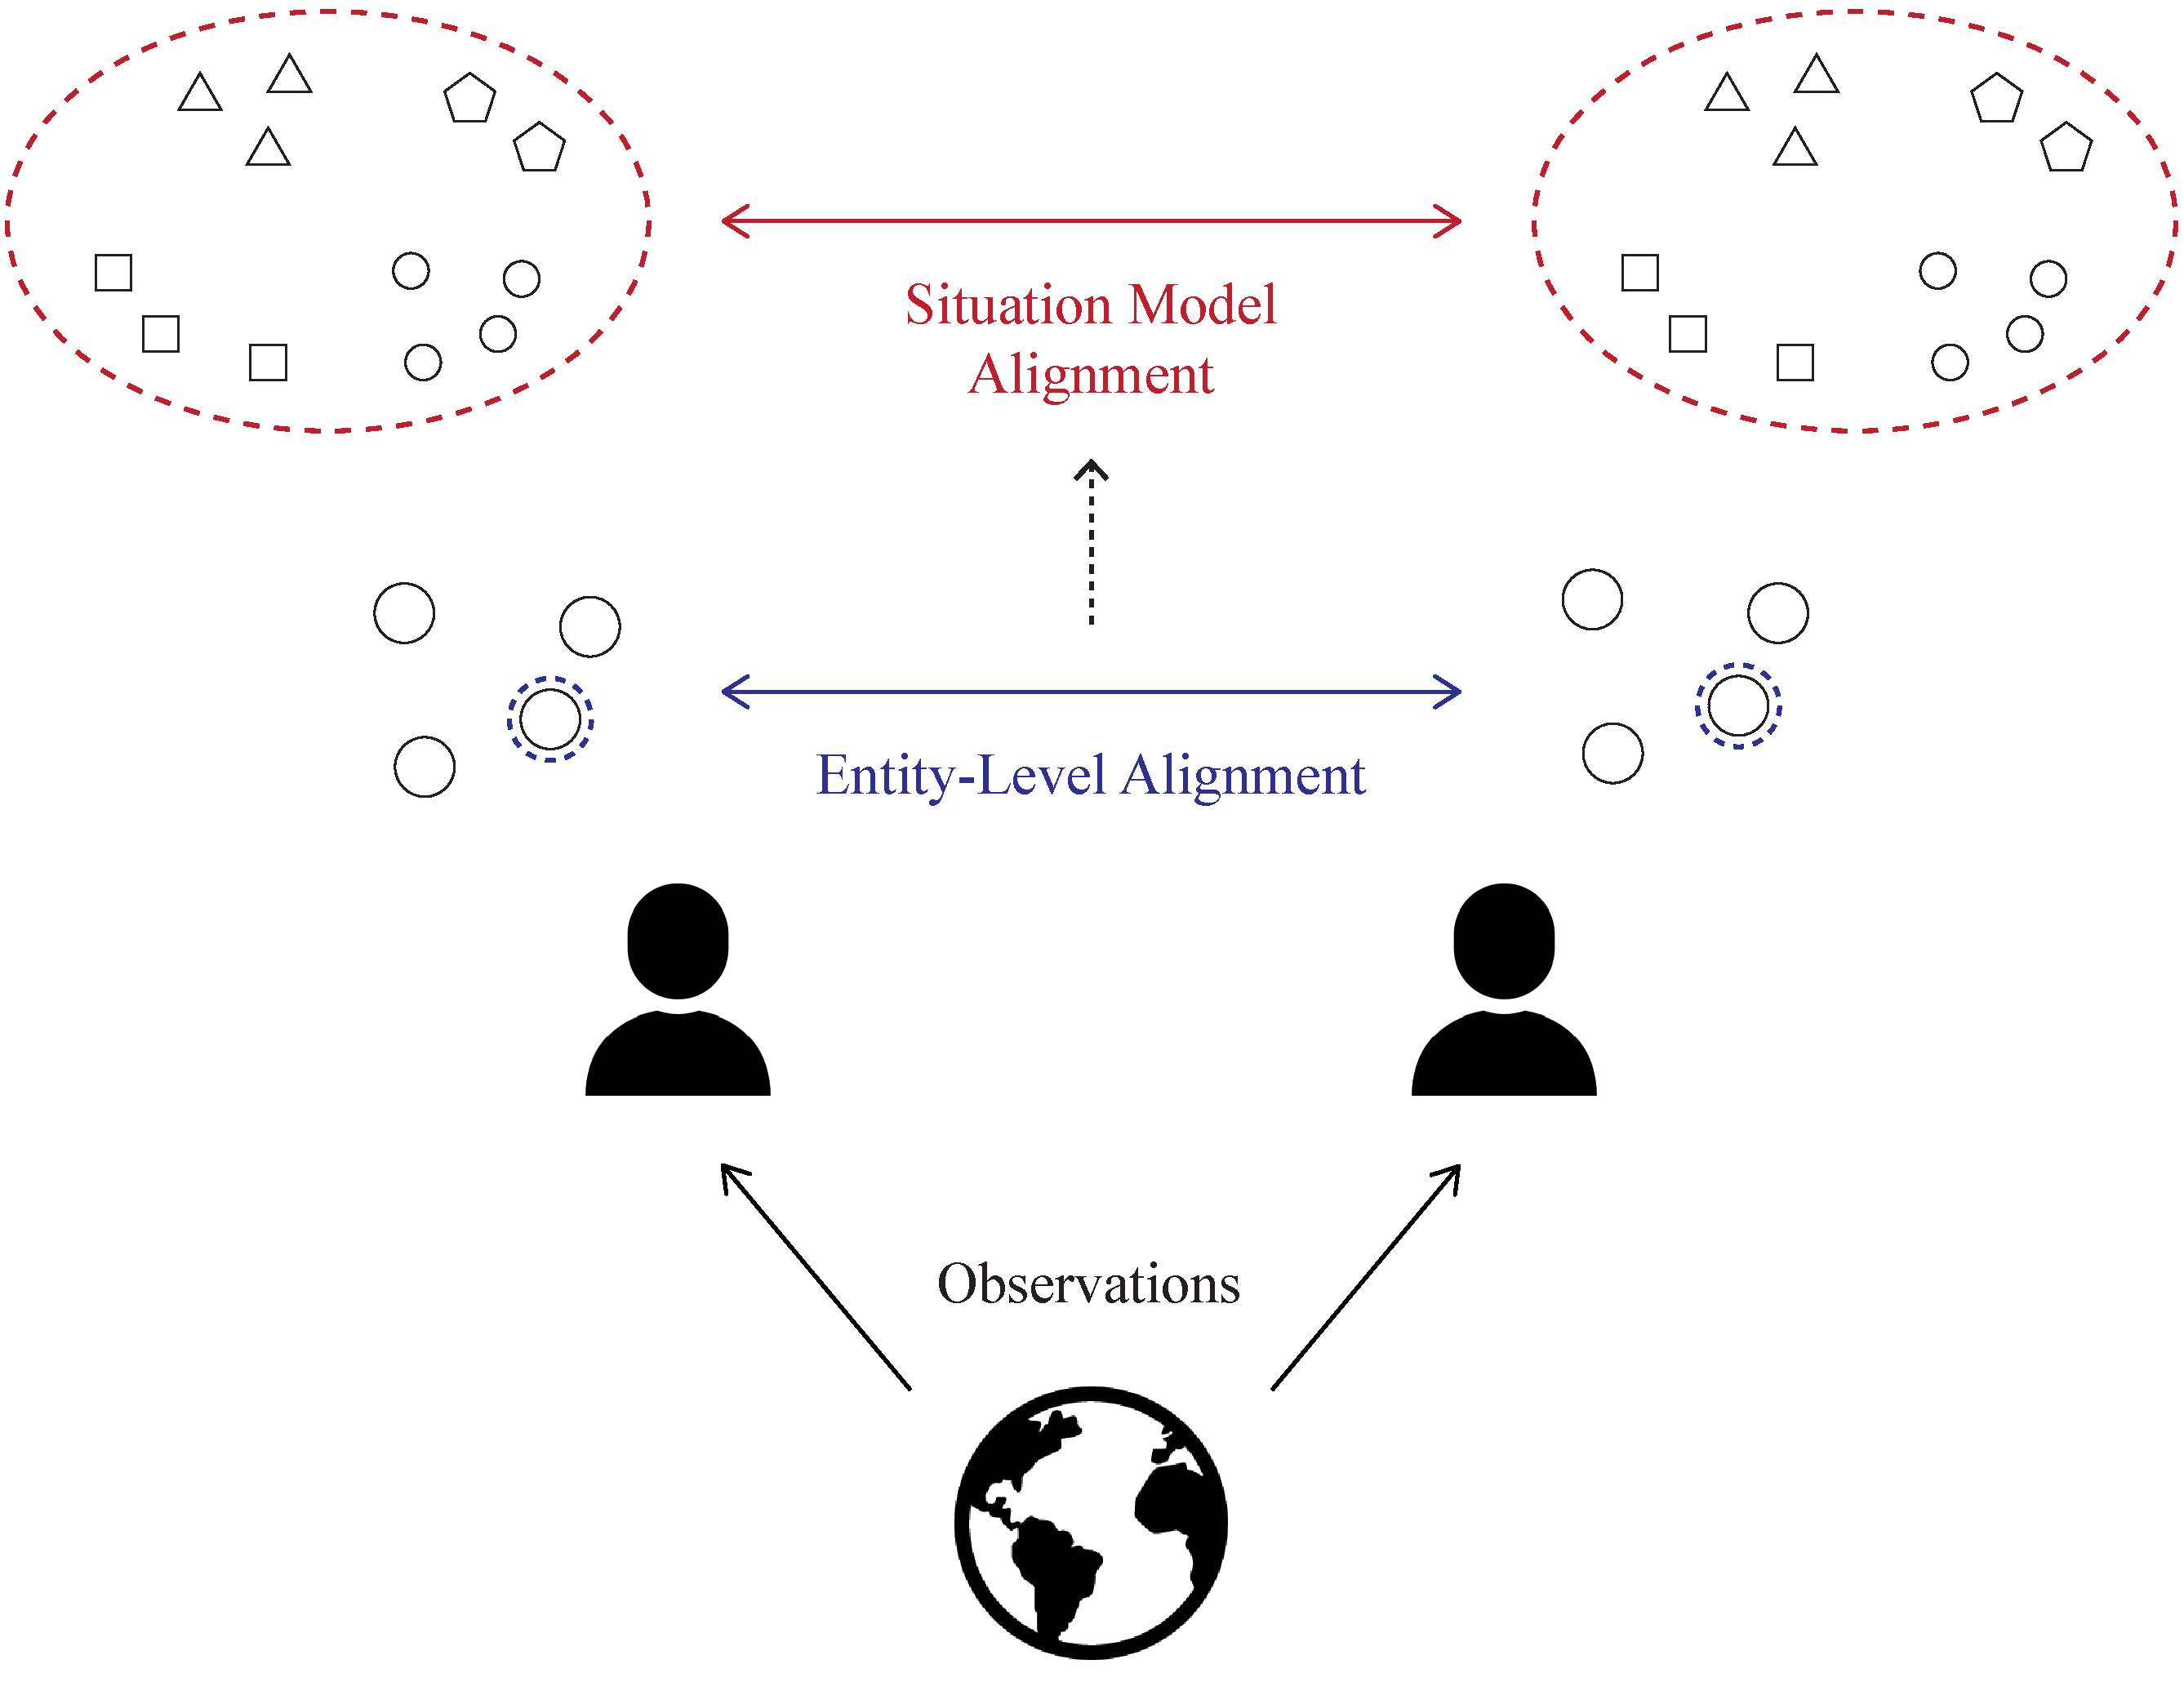
\includegraphics[width=\textwidth]{situation_models.pdf}
\caption{An illustration of the current task formulations (\textit{entity-level alignment}) and the desired task formulations (\textit{situation model alignment}).
}
\label{07_fig:situation_model_alignment}
\end{figure*}

If we were to study fully advanced common grounding, we expect task formulations which require the alignment of entire situation models will be critical (as illustrated in Figure \ref{07_fig:situation_model_alignment}). To be specific, we need appropriate task designs which require alignment at all conceivable dimentions (not only \textit{space} and \textit{time} but also \textit{causality}, \textit{intentionality} and \textit{protagonists}). We also need task formulations which enable reliable evaluation of the accurate situation model alignment (rather than entity-level alignment). These requirements are much more demanding, but there are several potential solutions. One approach is to carefully design questions to test whether the situation models are correctly aligned, as similarly proposed in the reading comprehension literature \citep{sugawara-etal-2021-benchmarking}. For instance, after (or in the middle of) the conversation, we can ask each interlocutor some questions that require the answers to be coordinated: e.g. ``what event do you (and your partner) expect if the player had not scored an own goal?'' or ``what do you (and your partner) believe the intention of the player was?'', where alignment of situation models at the \textit{causal} (\textit{counterfactual}) dimension and \textit{intentionality} dimension is required, respectively. We leave the exploration of specific task designs, evaluation metrics and dataset collection as an important avenue of future work.

\section{Improving Common Grounding}
\label{07_sec:advanced_common_grounding_models}

Throughout this thesis, we have proposed several approaches to improve common grounding in data-driven dialogue systems: such as multi-task training with reference resolution (Chapter \ref{04_chp:interpretation}) and pretraining on a related dataset (Chapter \ref{06_chp:task_generalization}). However, we can conceive of three major approaches to further improve their performances.

One approach is to make the model learn from the task success and failure based on \textit{reinforcement learning} \citep{sutton2018reinforcement}. This can be realized through an actual interaction with the human players (e.g. crowd workers) but also by repeatedly playing the task against itself, known as \textit{selfplay} \citep{silver2016mastering}. The latter approach is much cheaper and more scalable, hence widely applied in dialogue domains with symmetric speaker roles \citep{lewis-etal-2017-deal,DBLP:conf/icml/YaratsL18,jang2020bayes}. The upside is that we can expect the models to learn to avoid ineffective strategies, such as underspecification and premature guessing. However, the downside is that they can potentially diverge from natural language \citep{kottur-etal-2017-natural}, making communication with humans more difficult and unreliable.

We also expect the incorporation of \textit{pragmatic reasoning} to be a fruitful area of future research. One representative approach is the \textit{Rational Speech Act} (\textit{RSA}) framework \citep{Goodman2016PragmaticLI}, which has been applied in both continuous \citep{monroe2017colors,mcdowell-goodman-2019-learning} and partially-observable domains \citep{Hawkins2021TheDO}. However, application in \textit{interactive} and \textit{dynamic} domains would involve additional complexities that need to be taken into account, such as the dependencies on dialogue history and previous common ground.

Finally, we can study wider variety of model architectures and pretraining datasets. For instance, we have considered the observations to be in \textit{structured} format (e.g. based on xy coordinates), but we can also extract \textit{raw} visual features by directly treating them as images or videos \citep{suhr2017corpus,iki2020language}. In the latter case, we can apply various techniques from CV and NLP, including image/video processing methods \citep{Carreira2017QuoVA,wang2018non,dosovitskiy2021an}, vision-language grounding models \citep{lu2019vilbert,le-etal-2020-bist} and pretraining on large-scale, open domain datasets \citep{krishna2017visual,sharma-etal-2018-conceptual}. Note that the entity-level representation of the observation (required in our baselines) can be obtained from raw visual features as well, e.g. by utilizing the object detectors \citep{NIPS2015_14bfa6bb,redmon2016you} and trackers \citep{tracktor_2019_ICCV,wang2020towards}. Lastly, we can replace the \textit{dialogue encoders} of our baselines based on the transformer architectures \citep{NIPS2017_3f5ee243}, which have become the mainstream approch in language and dialogue modelling \citep{devlin-etal-2019-bert,lewis-etal-2020-bart,zhang-etal-2020-dialogpt}.


\section{Real-World Applications}
\label{07_sec:real_world_applications}

Finally, we'd like to discuss the impact of our work on real-world applications. While our resources (OneCommon Corpus and Dynamic-OneCommon Corpus) are currently restricted to synthetic settings, the general ideas and strategies we have investigated are fundamental in many practical applications.

For instance, consider the case of \textit{item retrieval}, such as recommending a furniture by soliciting the user preferences (as in \citealp{moon-etal-2020-situated}). Since the user's taste can be very precise, this requires dealing with subtle nuances like ``do you have something that's \textit{a little more} white and round shaped?'' or partial replacements like ``I like its materials \textit{except for} the backrest''. Dealing with such expressions are critical under \textit{continuous} context and can be studied rigorously based on OneCommon Corpus. In addition, this setting can become \textit{partially-observable} in case the actual furniture is not visible to the user, e.g. when the item is out of stock or the user is talking to speech-based devices. On such occasions, the system needs to take into account the possibility of various misunderstandings to make the transaction accurate and reliable.

We can also illustrate the importance of \textit{dynamic} context based on a navigation task in commonplace environments, such as finding a lost child in an urban city. In reality, the \textit{target entity} (the child) may not stay in one place, so the routing directions can no longer be fixed and need to be \textit{updated} accordingly (as in ``now head more to the west'' or ``go back to the previous block''). Furthermore, the \textit{landmark entities} may not be stationary either and could be ephemeral (as in ``following the group of travelers'' or ``in the middle of the crowd''). The task may be trivial if the child is conspicuous with few distractors, but otherwise (e.g. with many pedestrians around), the descriptions need to be precise and distinguishing (as in ``wearing \textit{a little} darker shirt'', ``walking \textit{right} towards the station''). In order to study such (nuanced and pragmatic) spatio-temporal expressions and references to previous common ground, we expect Dynamic-OneCommon Corpus to be an essential proving ground for developing and analyzing various models.\footnote{Unfortunately, most of the existing navigation tasks focus on \textit{static} environments (e.g. static targets and landmarks): see Section \ref{06_sec:related_work} for further discussions.}

Overall, we expect our contributions to be critical for promoting reliable collaboration in real-world environments, which involve the advanced settings of \textit{continuous}, \textit{partially-observable} and \textit{dynamic} context.




